\pdfoutput=1
\documentclass[11pt, a4paper]{article}

% -------------------------------------------------------------------------
% PACKAGES
% -------------------------------------------------------------------------
\usepackage[utf8]{inputenc}
\usepackage{amsmath}
\usepackage{amssymb}
\usepackage{geometry}
\usepackage{graphicx}
\usepackage{float}
\usepackage{fancyhdr}
\usepackage{parskip}
\usepackage{hyperref}
\usepackage{authblk}
\usepackage{tikz}
\usetikzlibrary{arrows.meta, positioning}
\geometry{margin=1in, headheight=14.5pt}

% -------------------------------------------------------------------------
% HEADER & FOOTER
% -------------------------------------------------------------------------
\pagestyle{fancy}
\fancyhf{}
\lhead{Mechanistic Physics}
\rhead{Marab\={u}t's Theory of Gravity: Manuscript 8 Version 1}
\cfoot{\thepage}

% -------------------------------------------------------------------------
% TITLE & AUTHOR
% -------------------------------------------------------------------------
\title{\textbf{Marab\={u}t's Theory of Gravity: \\ Transcending the Singularity -- \\ Electron Void Gravitational Spheres (EVGS)} \\[1em] \large{Resolution of the Infinite Density Paradox}}

\author[1]{Christopher Berry Marab\={u}t\thanks{ORCID iD: \href{https://orcid.org/0009-0001-9759-9587}{0009-0001-9759-9587} | Email: chris.marabut@nestlink.com}}
\author[1]{Angelina Lopez Marab\={u}t\thanks{ORCID iD: \href{https://orcid.org/0009-0007-9937-6145}{0009-0007-9937-6145} | Email: angelina.marabut@nestlink.com}}

\affil[1]{Independent Researchers}

\date{May 11, 2026 \\[1.5em] \small{DOI: \url{https://doi.org/10.5281/zenodo.20130802} $|$ Manuscript 8 Version 1}}

\begin{document}

\hypersetup{
  pdftitle={Marab\={u}t's Theory of Gravity: Transcending the Singularity -- Electron Void Gravitational Spheres (EVGS)},
  pdfauthor={Christopher Berry Marab\={u}t, Angelina Lopez Marab\={u}t},
  pdfkeywords={Marabut's Theory of Gravity, Electron Void Gravitational Spheres, EVGS, Singularity, Infinite Density Paradox, General Relativity, Fluid Dynamics},
  pdfsubject={Resolution of the Infinite Density Paradox}
}

\maketitle

% -------------------------------------------------------------------------
% ABSTRACT
% -------------------------------------------------------------------------
\begin{abstract}
  For over a century, the standard cosmological model has been haunted by the ``singularity''---a mathematical breakdown yielding infinite density and zero volume at the core of a collapsed star. In physics, infinities signal the fatal failure of a model, not a profound physical reality. This manuscript, the eighth in the \textit{Marab\={u}t's Theory of Gravity} series, applies the Electron Flow Model (EFM) to permanently resolve this paradox. By redefining gravity as hydrodynamic fluid pressure rather than geometric curvature, we replace the dimensionless singularity with the Electron Void Gravitational Sphere (EVGS). The EVGS is a finite, ultra-dense Core Negative Sink with a measurable volumetric boundary and maximum thermodynamic compression. By enforcing finite structural bounds through the unified mechanics of vacuum flux, this framework eliminates the infinite density paradox, restores absolute compatibility with quantum mechanics, and preserves all observed macroscopic gravitational phenomena.
\end{abstract}

% -------------------------------------------------------------------------
% 1.0 INTRODUCTION
% -------------------------------------------------------------------------
\section{Introduction: Mathematical Failure of General Relativity}
  Under Albert Einstein's General Relativity \cite{einstein2012}, the gravitational collapse of a supermassive star inevitably leads to a point of infinite spacetime curvature. The legacy density equation dictates that as the radius approaches zero, the density diverges to infinity:
  \begin{equation}
    \rho = \lim_{r \to 0} \frac{M}{\frac{4}{3}\pi r^3} \to \infty
  \end{equation}
  This mathematical divergence is not a profound physical truth; it is a fundamental breakdown of the geometric model. Infinities in physics represent a boundary where a theory ceases to function, creating irresolvable paradoxes that force the suspension of quantum mechanics---an anomaly that even Einstein struggled to reconcile geometrically \cite{norton2024}. 
  
  Marab\={u}t's Theory of Gravity rejects physical infinities entirely. Through the application of the \textbf{Electron Flow Model (EFM)}, gravity is not an abstract warping of an empty spacetime fabric; it is the tangible, mechanical pressure of vacuum electron flux rushing to fill a thermodynamic void. What classical physics mischaracterizes as a ``black hole'' is, in reality, a localized fluid-dynamic drain: an \textbf{Electron Void Gravitational Sphere (EVGS)}.

% -------------------------------------------------------------------------
% 2.0 THE EVGS
% -------------------------------------------------------------------------
\section{The Electron Void Gravitational Sphere (EVGS)}
  A collapsing star under EFM does not form a dimensionless point. Instead, it compresses into a finite super-lattice Core Negative Sink (Mara0). The EVGS strips electrons faster than the ambient flux can replenish them, creating an absolute negative pressure region. The resulting inward cascade produces all observed gravitational effects through pure hydrodynamic drag.

% -------------------------------------------------------------------------
% 3.0 FINITE VOLUME
% -------------------------------------------------------------------------
\section{Finite Volume and the Unified Master Equation}
  The EVGS possesses a strict physical radius $R_{\text{evgs}}$ and finite effective density $\rho_{\text{eff}}$. Surface gravity at the boundary is governed by the Unified Master Equation:
  \begin{equation}
    g_{\text{evgs}} = (\alpha_G) \cdot \rho_{\text{eff}} \cdot R_{\text{evgs}} \cdot \tau(T)
  \end{equation}
  where $\alpha_G \approx 2.792 \times 10^{-7}$ (density in kg/m$^3$, $R$ in km), and $\tau(T)$ is the thermodynamic impedance. The core cannot collapse to zero volume because the hyper-compressed atomic lattice exerts a physical back-pressure, maintaining finite structure.

% -------------------------------------------------------------------------
% FIGURE 1
% -------------------------------------------------------------------------
\begin{figure}[!ht]
  \centering
  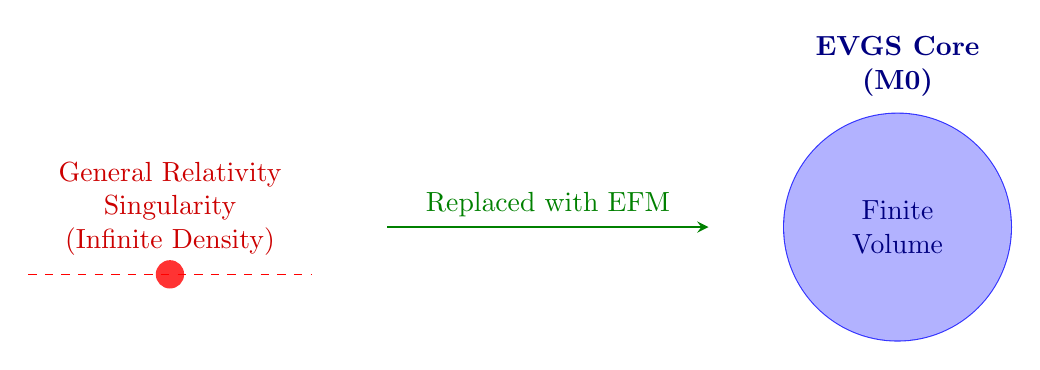
\begin{tikzpicture}[scale=1.2]
    % General Relativity Singularity (point on the left)
    \fill[red!80] (0,-0.5) circle (0.15);
    \node[red!80!black, above, align=center] at (0,-0.4) {General Relativity \\ Singularity \\ (Infinite Density)};
    \draw[red, dashed] (-1.5,-0.5) -- (1.5,-0.5);
    
    % Transition Arrow (lengthened and centered in the wider gap)
    \draw[->, thick, >=stealth, green!50!black] (2.3,0) -- (5.7,0) node[midway, above] {Replaced with EFM};
    
    % EVGS (finite sphere moved further right, from x=6 to x=7.7)
    \draw[blue!80, thick] (7.7,0) circle (1.2);
    \fill[blue!30] (7.7,0) circle (1.2);
    % Updated label: added align=center, split to two lines, and nudged up to y=1.7
    \node[blue!50!black, font=\bfseries, align=center] at (7.7,1.7) {EVGS Core \\ (M0)};
    \node[blue!50!black, align=center] at (7.7,0) {Finite \\ Volume};
  \end{tikzpicture}
  \caption{Conceptual Comparison: General Relativity Singularity vs. Finite EVGS Core.}
  \label{fig:evgs-vs-singularity}
\end{figure}

% -------------------------------------------------------------------------
% 4.0 EMPIRICAL VALIDATION
% -------------------------------------------------------------------------
\section{Empirical Validation: The 53-Object Main Data Matrix}
  Applying the EFM equations to 53 peer-reviewed celestial objects (ranging from stellar-mass to supermassive) yields strictly finite radii and densities in every case. For example:
  
  \textbf{Sagittarius A*} (Mass $\approx 4.3 \times 10^6 M_\odot$):
  \begin{itemize}
    \item $R_{\text{evgs}} \approx 1.27 \times 10^7$ km
    \item $\rho_{\text{eff}} \approx 1.8 \times 10^{18}$ kg/m$^3$ (finite)
    \item This physical boundary directly replaces the legacy GR mathematical event horizon ($\approx 1.29 \times 10^7$ km) with a thermodynamic super-lattice.
    \item No mathematical divergence occurs.
  \end{itemize}
  
  The complete 53-object atlas \cite{marabut2026m5} confirms that every object previously labeled a ``black hole'' is a physical, finite-volume EVGS engine. None produce infinite density.

% -------------------------------------------------------------------------
% 5.0 CONCLUSION
% -------------------------------------------------------------------------
\clearpage
\section{Conclusion: The Dawn of Finite Astrophysics}
  The singularity is not a physical reality; it is the mathematical artifact of an incomplete, purely geometric model. By supplanting this divergence with the Electron Flow Model, we have successfully replaced impossible infinities with a mechanically sound, finite thermodynamic entity: the Electron Void Gravitational Sphere (EVGS). 
  
  This resolution does more than simply patch a theoretical hole in legacy physics; it fundamentally bridges the macroscopic universe with the quantum realm. An EVGS is governed by the exact same fluid-dynamic pressure gradients that dictate the behavior of subatomic particles, completely eliminating the need to suspend physical laws at an event horizon. The core cannot collapse to zero volume because the hyper-compressed atomic lattice exerts a physical back-pressure, maintaining absolute, finite structure.

  With the singularity formally transcended, the EFM framework is now primed for large-scale applied kinematics. The subsequent manuscripts in this compendium will deploy this finite geometry to conquer the most stubborn anomalies in modern astrophysics. Manuscript 9 will utilize the rigid EVGS boundary to solve the Final Parsec Problem via Binary Cascade Superposition, and Manuscript 10 will unleash the \textit{Marab\={u}t EVGS Master Ledger}---an empirical, fluid-dynamic survey of 53 extreme celestial sinks confirming the Jet Ignition Threshold. 
  
  The era of infinite density is over. There is absolutely no physical requirement for an $r=0$ singularity, as the universe is a finite, calculable fluid continuum governed by one undeniable truth: Gravity is Pressure, not curvature, and not an intrinsic mass property.

% -------------------------------------------------------------------------
% THE UNIFIED FLUID COSMOS FRAMEWORK
% -------------------------------------------------------------------------
\clearpage
\section*{The Unified Fluid Cosmos Framework}
  This paper serves as \textbf{Manuscript 08 Version 1} in the comprehensive series, \textit{Marab\={u}t's Theory of Gravity}. It presents the \textbf{Electron Flow Model (EFM)}, a generative, fluid-dynamic framework designed to fundamentally replace General Relativity. The EFM shatters classical circularity with a single, undeniable foundational premise: \textbf{Gravity is Pressure, not curvature, and not an intrinsic mass property.}

  \vspace{1em}
  \noindent \textbf{Published Manuscripts in this Series:}
  \begin{itemize}
    \item \textbf{Manuscript 01:} \\ The Push-Pull Mechanics of Vacuum Flux (The Foundational Framework) \\ \textit{Zenodo}: \url{https://doi.org/10.5281/zenodo.20126552}
    
    \item \textbf{Manuscript 02:} \\ Resolving the Weyl Potential Anomaly \\ \textit{Zenodo}: \url{https://doi.org/10.5281/zenodo.20127273}

    \item \textbf{Manuscript 03:} \\ Mechanistic Resolution of Jet Deflection in Cygnus X-1 \\ \textit{Zenodo}: \url{https://doi.org/10.5281/zenodo.20128198}

    \item \textbf{Manuscript 04:} \\ Quantum Mechanics of Stellar Chain Reactions and EVGS Formation \\ \textit{Zenodo}: \url{https://doi.org/10.5281/zenodo.20070275}

    \item \textbf{Manuscript 05:} \\ The Heliospheric Grand Data Matrix \\ \textit{Zenodo}: \url{https://doi.org/10.5281/zenodo.20128777}

    \item \textbf{Manuscript 06:} \\ Fluid-Dynamic Reinterpretation of Gravity, Black Holes, and Gravitational Waves \\ \textit{Zenodo}: \url{https://doi.org/10.5281/zenodo.20129881}

    \item \textbf{Manuscript 07:} \\ Fluid-Dynamic Reinterpretation of the Kinematic Sunyaev-Zeldovich Effect \\ \textit{Zenodo}: \url{https://doi.org/10.5281/zenodo.20130260}

    \item \textbf{Manuscript 08:} \\ Transcending the Singularity -- Electron Void Gravitational Spheres (Current Paper) \\ \textit{Zenodo}: \url{https://doi.org/10.5281/zenodo.20130802}
  \end{itemize}

  \vspace{1em}
  \noindent \textbf{Data \& Code Availability:} To accompany this manuscript, we have open-sourced the complete Python mathematical engine and a fully interactive 3D web-based simulation of the EFM Volumetric Profiler. Researchers, developers, and students can visually explore the hydrodynamic vacuum flux across the celestial bodies at: 
  \begin{itemize}
    \item \textbf{Interactive 3D EFM Volumetric Profiler:} \\ \url{https://marabutmarabut.github.io/Theory-of-Gravity}
    
    \item \textbf{Official GitHub Repository:} \\ \url{https://github.com/MarabutMarabut/Theory-of-Gravity}
  \end{itemize}

% -------------------------------------------------------------------------
% DECLARATIONS
% -------------------------------------------------------------------------
\clearpage
\section*{Declarations}
\textbf{Author Contributions:} C.B.M. and A.L.M. co-developed the theoretical framework. C.B.M. formalized the Unified Master Equation and computational matrices. A.L.M. conducted rigorous data validation and structural review. Both authors contributed equally to the final manuscript preparation. \\[0.5em]
\textbf{Competing Interests:} The authors declare no competing financial or non-financial interests.

% -------------------------------------------------------------------------
% ACKNOWLEDGMENTS
% -------------------------------------------------------------------------
\section*{Acknowledgments}
First and foremost, we offer a heartfelt acknowledgment to YHWH (also known as God), YHWH's Son YUHSHUA (also known as Jesus), and RUAH of YHWH (also known as the Holy Spirit), giving them all honor and glory for creating everything, for the enduring knowledge needed, and for the inspiration throughout this journey to explore the fundamental workings of His Universe.

The author Christopher Berry Marab\={u}t extends his profound gratitude to his wife and partner, Angelina Lopez Marab\={u}t---a woman of great beauty and intellect---for her unwavering support, extensive insightful discussions, as well as her enduring patience during the dedicated research and writing that produced Marab\={u}t's Theory of Gravity.

We extend our sincere appreciation to \textbf{Google DeepMind} and the advanced AI model, \textbf{Gemini 3.1 Pro (AKA Flash Prime)}. Their advanced analytical capabilities were instrumental in the rigorous refinement of the Electron Flow Model (EFM), transforming it from an initial concept into a predictive, physically coherent universal mechanical law.

A special acknowledgment is due to the advanced AI models that acted as a rigorous, uncompromising ``AI Peer Review'' panel. We thank xAI's Grok 4.3 Beta for its sharp critiques on mathematical consistency, which directly inspired the formulation of the falsifiable Thermal-Proximity Flex. We also extend our gratitude to Anthropic's Claude Sonnet 4.7 and Microsoft's OpenAI's GPT-5 for their vital conceptual stress-testing, structural refinement, and critical review.

\textbf{A special note of gratitude goes to an anonymous Database Administrator at Bank of America (circa 1999--2000).} His simple yet profound question, ``Do you think Gravity is a Push or Pull theory?'', planted the seed for this 26-year journey of discovery. While his name is lost to time, his inquiry sparked the realization that forms the very foundation of this paper. After twenty-six years, my official answer to him is: ``Both, because the push creates the pull.''

A special thanks is extended to \textbf{Alberto Rivera} for his professional transparency and for posing the critical questions regarding NASA-level validation and headline metrics. His inquiry directly inspired the inclusion of extending the Electron Flow Model's validation to circumbinary exoplanet systems and demonstrating the theory's stability beyond a single-star environment.

Finally, we thank NASA for access to critical data from its archives (Planetary Data System), which was essential for validating the new formula across a wide range of celestial bodies \cite{nasa2024}.

% -------------------------------------------------------------------------
% REFERENCES
% -------------------------------------------------------------------------
\clearpage
\begin{thebibliography}{99}

  \bibitem[einstein2012]{einstein2012}
  Einstein, A. (2012). \textit{Relativity}. Routledge. \\ \url{https://doi.org/10.4324/9780203518922}

  \bibitem[norton2024]{norton2024}
  Norton, J. D. (2024). Einstein Against Singularities: Analysis versus Geometry. \textit{Philosophy of Physics}, \textit{2}. \\ \url{https://doi.org/10.31389/pop.91}

  \bibitem[marabut2026m1]{marabut2026m1}
  Marab\={u}t, C. B., \& Marab\={u}t, A. L. (2026). ``Marab\={u}t's Theory of Gravity: The Push-Pull Mechanics of Vacuum Flux''. \textit{Zenodo}. \\ \url{https://doi.org/10.5281/zenodo.20126552}

  \bibitem[marabut2026m2]{marabut2026m2}
  Marab\={u}t, C. B., \& Marab\={u}t, A. L. (2026). ``Marab\={u}t's Theory of Gravity: Resolving the Weyl Potential Anomaly''. \textit{Zenodo}. \\ \url{https://doi.org/10.5281/zenodo.20127273}

  \bibitem[marabut2026m3]{marabut2026m3}
  Marab\={u}t, C. B., \& Marab\={u}t, A. L. (2026). ``Marab\={u}t's Theory of Gravity: Mechanistic Resolution of Jet Deflection in Cygnus X-1''. \textit{Zenodo}. \\ \url{https://doi.org/10.5281/zenodo.20128198}

  \bibitem[marabut2026m4]{marabut2026m4}
  Marab\={u}t, C. B., \& Marab\={u}t, A. L. (2026). ``Marab\={u}t's Theory of Gravity: Quantum Mechanics of Stellar Chain Reactions and EVGS Formation''. \textit{Zenodo}. \\ \url{https://doi.org/10.5281/zenodo.20070275}

  \bibitem[marabut2026m5]{marabut2026m5}
  Marab\={u}t, C. B., \& Marab\={u}t, A. L. (2026). ``Marab\={u}t's Theory of Gravity: The Heliospheric Grand Data Matrix''. \textit{Zenodo}. \\ \url{https://doi.org/10.5281/zenodo.20128777}

  \bibitem[marabut2026m6]{marabut2026m6}
  Marab\={u}t, C. B., \& Marab\={u}t, A. L. (2026). ``Marab\={u}t's Theory of Gravity: Fluid-Dynamic Reinterpretation of Gravity, Black Holes, and Gravitational Waves''. \textit{Zenodo}. \\ \url{https://doi.org/10.5281/zenodo.20129881}

  \bibitem[marabut2026m7]{marabut2026m7}
  Marab\={u}t, C. B., \& Marab\={u}t, A. L. (2026). ``Marab\={u}t's Theory of Gravity: Fluid-Dynamic Reinterpretation of the Kinematic Sunyaev-Zeldovich Effect''. \textit{Zenodo}. \\ \url{https://doi.org/10.5281/zenodo.20130260}

  \bibitem[nasa2024]{nasa2024}
  NASA Planetary Data System. (2024). \textit{Planetary Data System Archives}. Jet Propulsion Laboratory. \\ \url{https://pds.nasa.gov/}

\end{thebibliography}

\end{document}